\documentclass[11pt]{exam}
\usepackage{listings}
\lstset{language=Java}
\usepackage{pdfsync}

\textwidth = 6.5 in
\textheight = 8.5 in
\oddsidemargin = 0.0 in
\evensidemargin = 0.0 in
\topmargin = 0.0 in
\headheight = 0.0 in
\headsep = 0.25 in
\parskip = 0.15in
\parindent = 0.0in

\clubpenalty=10000
\widowpenalty=10000
\sloppy
%
%  Created by Mike Helmick on 2005-12-02.
%  Copyright (c) 2005 Mike Helmick. All rights reserved.
%
%

\newif\ifpdf
\ifx\pdfoutput\undefined
\pdffalse % we are not running PDFLaTeX
\else
\pdfoutput=1 % we are running PDFLaTeX
\pdftrue
\fi

\ifpdf
\usepackage{subfigure}
\usepackage[pdftex]{graphicx}
\else
\usepackage{graphicx}
\fi

%
%  Update these values for running headers
%
\firstpageheader{\bf\Large CSA 274-A}{\bf\Large FINAL EXAM}{\bf\Large
  2006 }
\runningheader{CSA 274-A/Spring 2006}{Miami University}{Final Exam}
\addpoints

\begin{document}


\vspace{3.0in}
\begin{center} 
  \fbox{\fbox{\parbox{5.5in}{\centering
      Miami University - CSA274-A - Spring 2006 - Final Exam 
\par
      There are \numquestions\  questions for a total of  \numpoints\ points.}}}
\end{center} 

% setup standard options for the including code fragments
\lstset{language=Python,numbers=left}

\vspace{0.1in} 
\hbox to \textwidth{Name:\enspace\hrulefill} 

\section*{Instructions}
Please read through this entire exam very carefully before starting.
\par
You may use one sheet of paper no larger than size 8.5" by 11" in size, double sided, of pre-prepared material.   This sheet must be prepared by you and not shared with anyone else. \newline
Other than that, this exam is closed notes and closed books.
\par
All work must be written on the exam pages in order to be graded.   Any scrap paper used, must be the scrap paper provided during the exam period.
\par
For programming questions: Please be as accurate as possible with your Java syntax: this includes appropriate use of braces, semicolons, and the proper use of upper/lowercase letters.  
\par
No electronic devices may be used during the exam: this includes calculators, iPods, PDAs, and cellular phones.
\par
You have 120 minutes to complete the exam.  
\par
There are \numpoints\ possible points, but the exam will be graded out of 200 points.
\par
{\bf Good Luck!}


\pagebreak

% Questions start here:
\begin{questions}

\question Given the following code for generic data structure:
\begin{lstlisting}
public class Building<E,T> {
    private E entrance;
    private T elevator;

    public Building() {}

    // .. remaining valid class definition 	 
}	
\end{lstlisting}
\begin{parts}
	\part[3] The symbols {\tt E} and {\tt T} represent what? \makebox[2in]{\hrulefill}
	\part[3] Write the line of code to declare a variable named {\tt kregerHall} of type {\tt Building} where the generic class types used are {\tt DoubleDoor} and {\tt Slow}, the variable should be initialized by invoking the default constructor. \newline

\end{parts}

\newpage
\question[15] For array list, we discussed dynamically growing the list in the event that more space is needed.   It might also make sense to shrink the array to reclaim unused space.   Complete the {\tt shrink} method below to reclaim space {\it in the event that the items in the array are less than half of the capacity}, by reducing the capacity by half of the current capacity.

\begin{verbatim}
public class ArrayList<E> {
    private E[] data;
    private int size;

    // assume the rest of the class is listed and complete

    public E removeLast() {
        E rtn = data[--size];
        shrink();
        return rtn;
    }
	
    private void shrink() {
        // BEGIN ANSWER
		
	
	
	
	
	
	


	
	
	
	
	
	
	
	
	
	
	
	
	
	
        // END ANSWER
    }
}
\end{verbatim}

\newpage
\question[20] Tree traversals apply not only to binary trees and/or search trees, but to all trees.  For example, consider the tree in Figure \ref{fig:exampleTree}.   This is a tree in which any given node can have a variable number of children.   Traversals can also be performed using a stack data structure.  For example, to perform a {\bf preorder} traversal on a tree we can {\tt pop} the top node off of the stack, process it, {\tt push} all of the node's children on the stack (in reverse order) and repeat the process.   To bootstrap the algorithm, we push the root on to the stack and start the process.    A preorder traversal using a stack is an {\bf iterative} process and is {\it not recursive.}
\begin{figure}[htbp]
   \begin{center}
      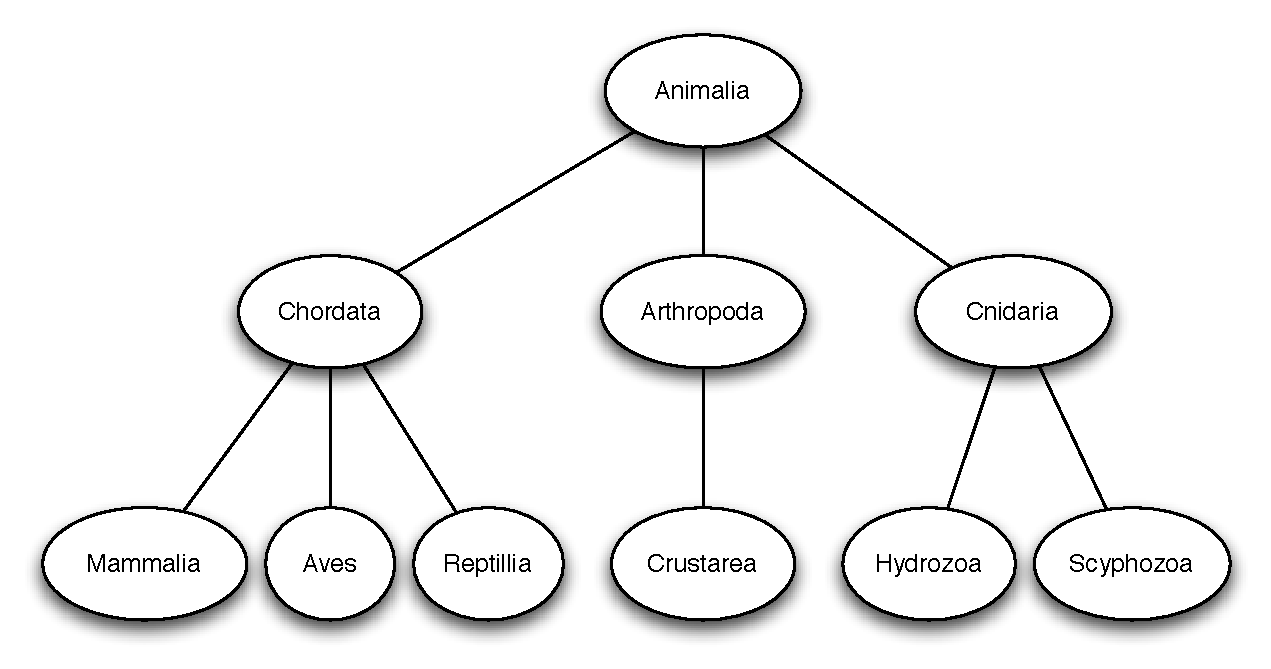
\includegraphics[width=6in]{animals}
   \end{center}
   \caption{Animal Kingdom Tree}
   \label{fig:exampleTree}
\end{figure}

For this question, you are to complete the iterative preorder traversal method using only what is provided (next page).
\newpage

\begin{verbatim}
public class GenericTree<E> {
    private Node<E> root;

    private static class Node<E> {
        private E data;
        private List<Node<E>> children = (List<Node<E>>) new ArrayList();
    }

    public List<E> preOrderTraversal() {
        List<E> results = new ArrayList<E>();

        // Stack has methods push(E), pop(), and isEmpty() - ignore exceptions
        Stack<Node<E>> stack = new Stack<Node<E>>();
        stack.push( root );
        // BEGIN ANSWER


























        // END ANSWER
        return results;
    }
}
\end{verbatim}
\newpage

\question[15] Code a recursive method for converting a {\bf string} of digits into the integer it represents.  For example ``1326458'' represents the integer 1,326,458.   For this; the input is a {\tt String}, the output is an {\tt int}, and your method should be named {\tt convertInt}.

\begin{verbatim}
public class Converter {

	private int convertDigit( char c ) {
		// ASSUME THAT THIS METHOD WORKS FOR CONVERTING A SINGLE DIGIT
	}

	// BEGIN ANSWER - you need to define the method(s) used
	
	
	
	
	
	
	
	
	
	
	
	
	
	
	
	
	
	
	
	
	
	
	
	
	
	
	
	
	
    // END ANSWER
}
\end{verbatim}

\newpage

\question Rank the following growth rates from the slowest rate of growth first to the fastest rate of growth (such that $O(a) < (b) < (c)$ etc...): $O(\log{n}), O(n), O(1), O(n^2), O(n!), O(n \: \log{n}) $
\begin{parts}
	\part[2] \makebox[4in]{\hrulefill}
	\part[2] \makebox[4in]{\hrulefill}
	\part[2] \makebox[4in]{\hrulefill}
	\part[2] \makebox[4in]{\hrulefill}
	\part[2] \makebox[4in]{\hrulefill}
	\part[2] \makebox[4in]{\hrulefill}
\end{parts}


\question[5] Convert the following code from explicit iterator use to Java (enhanced for loop.
\begin{lstlisting}
	List<Integer> list = new ArrayList<Integer>();
	fillList( list );
	
	// START converting here
	Iterator<Integer> iter = list.iterator();
	while( iter.hasNext() ) {
	   Integer thisInt = iter.next();
		System.out.println( thisInt );
	}
	// END converting here
\end{lstlisting}
\vspace{3in}
\newpage
\question[5] For a hash table of size $n$, using open addressing, and assuming that resizing is disabled.   What is the worst case running time for inserting into the hash table?  Why? {\it You may assume that the table will never allow more than $n-1$ elements in it.}
\vspace{3.0in}

\question[5] The AVL tree shown below has just had 67 inserted.  Show the proper rotation(s) to return the tree to balance, all nodes should have a balance of 0 with the process is complete.
\begin{figure}[htbp]
	   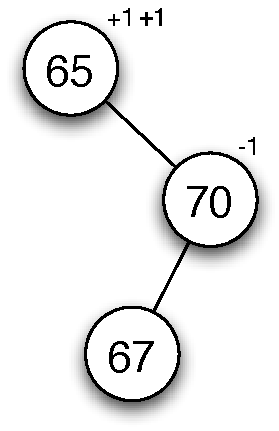
\includegraphics[width=2in]{final_rotate_question} 
\end{figure}
\newpage

e

\newpage
\question[12] Show the depth first search tree starting at node $B$.  Vertices should be selected in alphabetical order when there is more than 1 to choose from.   {\it Vertices should be processed in the order in which they are discovered.}
\begin{figure}[htbp]
	\begin{center}
	   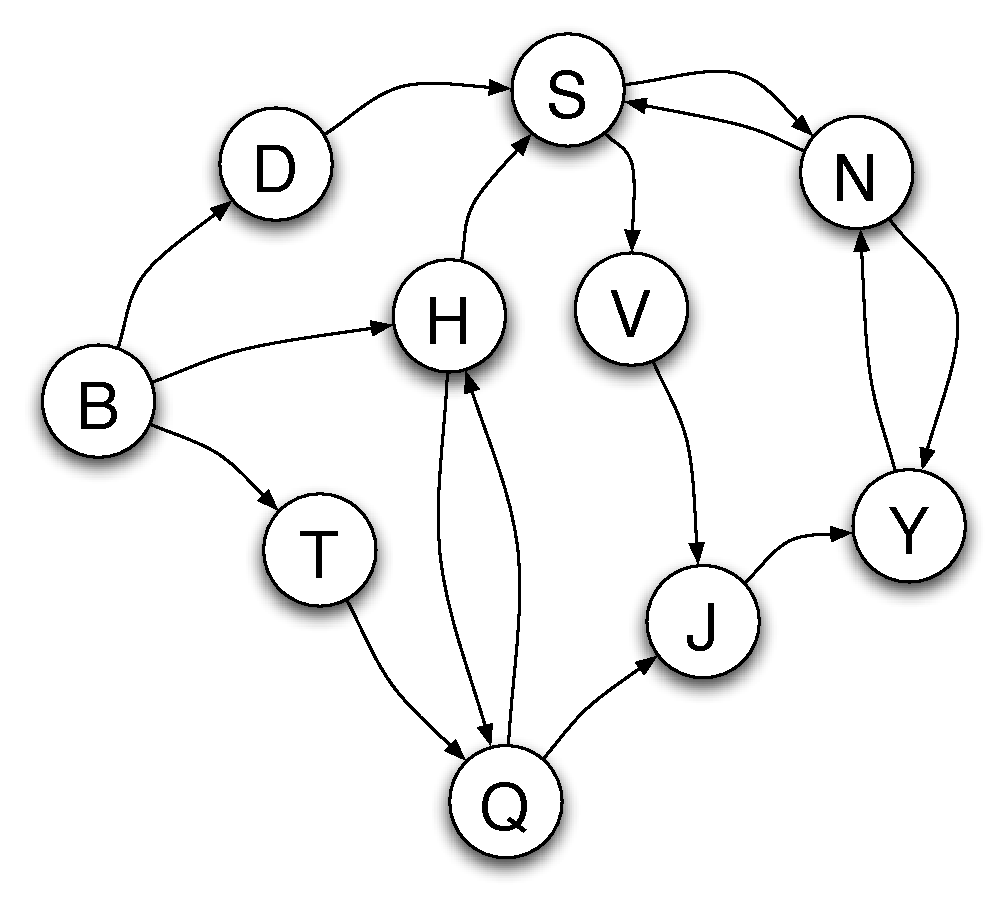
\includegraphics[width=5.5in]{final_graph_question}
	\end{center}   
	\label{fig:graph}
\end{figure}

\newpage
\question[20] We have discussed Prim's algorithm for building a minimum spanning tree.  With Prim's algorithm we grow a tree by selecting the next vertex that is closest to the current tree.
\par
Kruskal's algorithm is another important algorithm for calculating the minimum spanning tree in a graph.  Kruskal's algorithm works by selecting the {\it edge} with the lowest weight that (1) is not in the tree and (2) will not cause a cycle.  For example, in the graph below, the edge from $A \rightarrow C$ will be the first taken because it has the lowest weight of the unselected edges (initially all edges) and does not create a cycle.  
\par
A cycle is created when the edge to be added would be between two vertices that are already in the minimum spanning tree.   For Kruskal's algorithm, if an edge were to create a cycle, we simply disregard it and move on to the edge with the next lowest weight.
\par
For this question, show the minimum spanning tree in the below graph using Kruskal's algorithm.   Answer by indicating the order in which the edges are chosen to join the minimum spanning tree.
\begin{figure}[htbp]
	\begin{center}
	   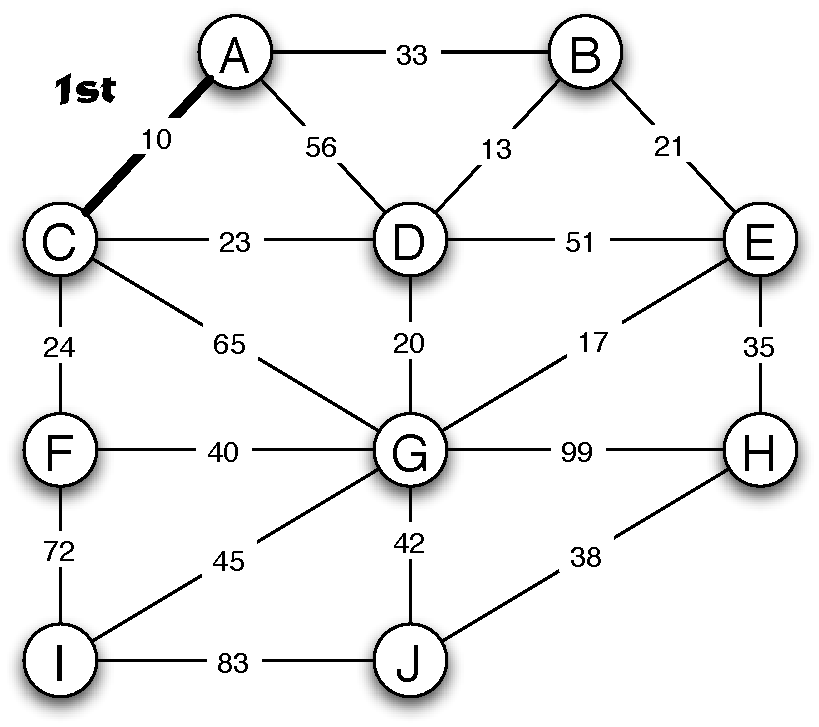
\includegraphics[width=6.0in]{final_mst_graph}
	\end{center}   
\end{figure}

\newpage
\question You are working on a new computer game with a team of programmers.   While the game is nearly complete, there is a problem with the game play.  The board is a undirected graph taking the form shown below.   A player can move their playing piece along any of the edges during their turn.
\begin{figure}[htbp]
	\begin{center}
	   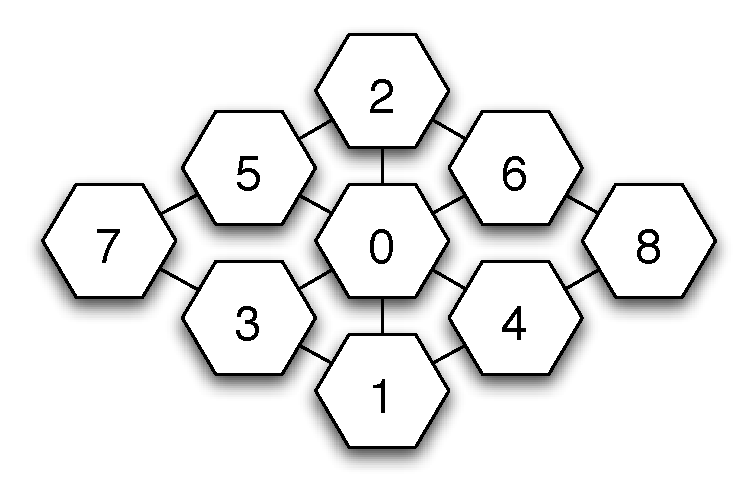
\includegraphics[width=3.15in]{final_game_question}
	\end{center}   
\end{figure}
One of the programmers on your team informs you that while playing the game, a player only seems to be able to move from one space to another if the number on the {\bf from square} is {\it lower} than the number on the {\bf to square}.  After running your JUnit tests on the game board class, you see that they are no longer working, so you print out the adjacency matrix that represents the graph of the board, and see this (and empty space indicates $0$ or no edge, and $1$ represents the presence of an edge): \newline
\begin{center}
\begin{tabular}{|c||c|c|c|c|c|c|c|c|c|} \hline
 X & 0 & 1 & 2 & 3 & 4 & 5 & 6 & 7 & 8 \\ \hline \hline
 0 &   & 1 & 1 & 1 & 1 & 1 & 1 &   &   \\ \hline
 1 &   &   &	& 1 & 1 &   &   &   &   \\ \hline
 2 &   &   &	&   &   & 1 & 1 &   &   \\ \hline
 3 &   &   &	&   &   &   &   & 1 &   \\ \hline
 4 &   &   &	&   &   &   &   &   & 1 \\ \hline
 5 &   &   &	&   &   &   &   & 1 &   \\ \hline
 6 &   &   &	&   &   &   &   &   & 1 \\ \hline
 7 &   &   &	&   &   &   &   &   &   \\ \hline
 8 &   &   &	&   &   &   &   &   &   \\ \hline
\end{tabular}
\end{center}


\begin{parts}
	\part[5] What's wrong with the graph representation in memory? \vspace{1.2in}
	\part[25] The team agrees on a quick fix where you will take the game board and correct the representation in memory using a small utility function (which they also ask you to write).   Fill in the details of this method on the following page.
\end{parts}

\newpage
\begin{verbatim}
public class GameBoard {
  private static final int SIZE = 9;
  private int[][] board = new int[size][size];

  public GameBoard() {
    initializeBoard();
    correctBoard(); // this is the method that you need to write
  }

  // ... the rest of the class

  private void correctBoard() {
    // BEGIN ANSWER

























    // END ANSWER
  }
}	
\end{verbatim}

\newpage
\question Merge sort can be easily split into two methods, a recursive merge sort method and a utility method to merge two sub-arrays back into a source array.   Complete the code for merge sort where the input array consists only of items that implement the {\tt Comparable} interfaces (that is, you must use the {\tt compareTo} method to determine their order).
\begin{parts}
  \part[10] Complete the code for the sort method.
  \part[15] Complete the code for the merge method.	
\end{parts}

\begin{verbatim}
public class MergeSort {
  public static  <T extends Comparable<T>> void sort( T[] array ) {










  }
  private static <T extends Comparable<T>> void merge(T[] output, T[] left, T[] right) {






















  }	
}
\end{verbatim}

\newpage
\question[15] Write a recursive method for finding the largest item in this linked list, noting that all items are {\it comparable} and thus have a {\it compareTo} method.

\begin{verbatim}
public class LinkedList<E extends Comparable> {
    private Node<E> root;
	
    private static class Node<E2 extends E> {
        private E2 data; 
        private Node<E2> next;
    }

    public E findLargest() {
        return findLargest(root);
    }
	
    private E findLargest( Node<E> root ) {
        // BEGIN ANSWER



















        // END ANSWER
    }
}
\end{verbatim}

\newpage
\question[15] Given the 2-3 Tree below, show the resultant tree if the value {\tt 30} is inserted.   You may either show the final tree or any intermediate steps that you find helpful.

\begin{figure}[htbp]
	\begin{center}
	   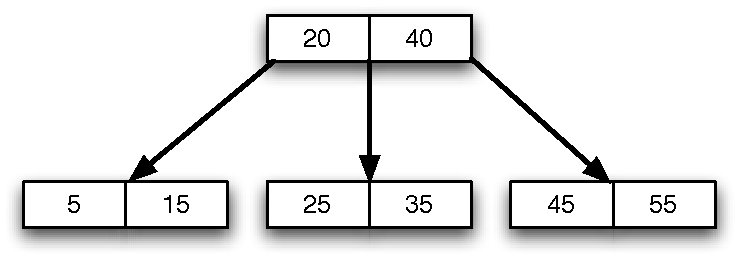
\includegraphics[width=4.5in]{final_23tree_insert}
	\end{center}   
\end{figure}

\end{questions}
\end{document}